\documentclass[12pt]{beamer}
\usetheme{Hannover}
\usepackage{graphicx}
\usepackage{booktabs}
\usepackage[english]{babel}
\usepackage{kotex}
%\usepackage[pdfencoding=auto]{hyperref}
\hypersetup{pdfencoding=auto}
\usepackage{ulem}
\usepackage[per-mode=symbol]{siunitx}
\sisetup{inter-unit-product =$\cdot$}
\usepackage{color}
\usepackage{ulem}
\usepackage{amsmath,amssymb}
\graphicspath{{images/}}
\title[\LaTeX - Day 0]{\LaTeX 입문 - Day 0}

\author{경기과학고 \TeX 사용자협회}
\institute[GSHSTeXSociety]{\url{latex.gs.hs.kr}}
\date{마지막 수정일 : \today}


%\AtBeginSection[]{
%	\begin{frame}
%		\vfill
%		\centering
%		\begin{beamercolorbox}[sep=8pt,center,shadow=true,rounded=true]{title}
%			\usebeamerfont{title}\insertsectionhead\par%
%		\end{beamercolorbox}
%		\vfill
%	\end{frame}
%}

\begin{document}

\begin{frame}
\titlepage % Print the title page as the first slide
\end{frame}

\section{What?}
\begin{frame}{\LaTeX 이란?}
	\begin{itemize}
		\item 개발
		\begin{itemize}
			\item Donald Knuth 에 의해 \TeX 개발됨(1978)
			\item \TeX 을 쉽게 사용하기 위한 매크로 : \LaTeX
			\item 발음 : [텍], [레이텍]
		\end{itemize}
		\item 특징
		\begin{itemize}
			\item 수식입력 기능, 자동 ToC\footnote{Table of Contents}, LoF\footnote{List of Figures}, LoT\footnote{List of Tables} 생성
			\item 편리한 labeling 및 referencing
			\item 많은 학회에서 tex 으로 논문을 투고받음
			\item 초기 설정 이후 내용 작성에만 집중 가능
			\item 논문, 발표자료, 시험지, 악보 등등... 만능!
		\end{itemize}
	\end{itemize}
\end{frame}
\begin{frame}{문서 편집기의 양대 산맥}
	What You See Is What You...
	\vfill
	\begin{columns}
		\begin{column}{0.5\textwidth}
			Get! \\
			\vfill
			우리가 보통 사용하는 한컴오피스, MS 워드. \\
			\begin{center}
				
\includegraphics[width=0.4\textwidth]{hanwordicon.jpg}
				~
				
\includegraphics[width=0.4\textwidth]{mswordicon.jpg}
			\end{center}
			
		\end{column}
		\begin{column}{0.5\textwidth}
			Mean! \\
			\vfill
			\textbf{나무위키}, HTML, \LaTeX \\
			\begin{center}
				
\includegraphics[width=0.4\textwidth]{namu.png}
				~
				
\includegraphics[width=0.4\textwidth]{htmlicon.png}
			\end{center}
		\end{column}
	\end{columns}
\end{frame}
\section{How?}
\begin{frame}{\TeX 설치하기}
	KTUG(Korean \TeX User Group)\footnote{한글 \TeX 사용자 그룹, [케이턱]}
	\begin{itemize}
		\item \TeX 사용 환경 조성 : TeXLive
		\item 한글을 사용하기 위한 TeXLive 가 koTeXLive
		\item 내려받기 - 설치 방법대로 따라간다.
		\item 용량이 약 2GB. 시간적 여유를 가지고 설치.
	\end{itemize}
	\TeX 문서 편집기
	\begin{itemize}
		\item TeXLive에서 기본 제공 : TeXWorks / TeXshop
		\item 하지만 TeXStudio\footnote{texstudio.org}가 훠---얼씬 편하다!
	\end{itemize}
\end{frame}
\section{Why?}
\begin{frame}{~}
	\vfill
	\centering
	\begin{beamercolorbox}[sep=8pt,center,shadow=true,rounded=true]{title}
		\Huge 그래서, 왜 \\ \LaTeX 을 쓰는거지?
	\end{beamercolorbox}
	\vfill
\end{frame}
\subsection{장점}
\begin{frame}{\LaTeX 의 장점}
	\LaTeX 의 장점들
	\begin{itemize}
		\item 수식 편집기로서는 수학에서는 \textbf{표준}
		\item 초기설정만 잘 해놓으면 노가다가 줄어듦.
		\begin{itemize}
			\item 차례, 그림/표 목차를 만들 때...명령어 하나로 끝!
			\item 참고문헌이 50개인데... 자동 인용순 정렬!
			\item `수정한다'에 대한 공포감(?) 전혀 없음
		\end{itemize}
		\item Cross-referencing : `그림 8a에 의하면...'
		\begin{itemize}
			\item 편하며, 실시간으로 `큰그림'이 보인다. 
		\end{itemize}
		\item 벡터 이미지(svg, eps, pdf) 손쉽게 첨부
		\begin{itemize}
			\item 훨씬 깔끔하다. 논문의 권위는 여기에서 출발.
		\end{itemize}
	\end{itemize}
\end{frame}
\begin{frame}{작업량}
	\begin{figure}[h]
		\centering
		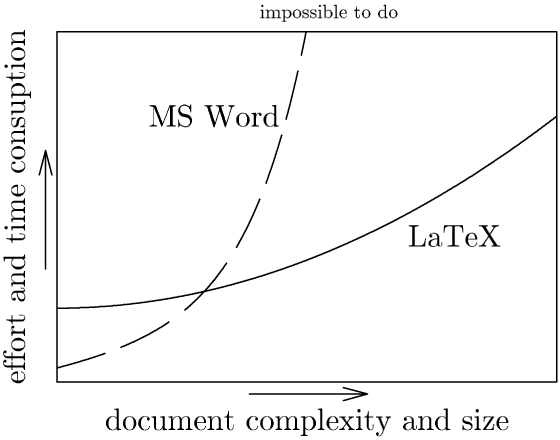
\includegraphics[width=\textwidth]{msword_vs_latex.png}
	\end{figure}
\end{frame}
\subsection{Examples}
\begin{frame}{예시 - 선형대수학 요약본}
	\framesubtitle{무려 100페이지! By 14129 황동욱 + 32기}
	\begin{figure}[h]
		\centering
		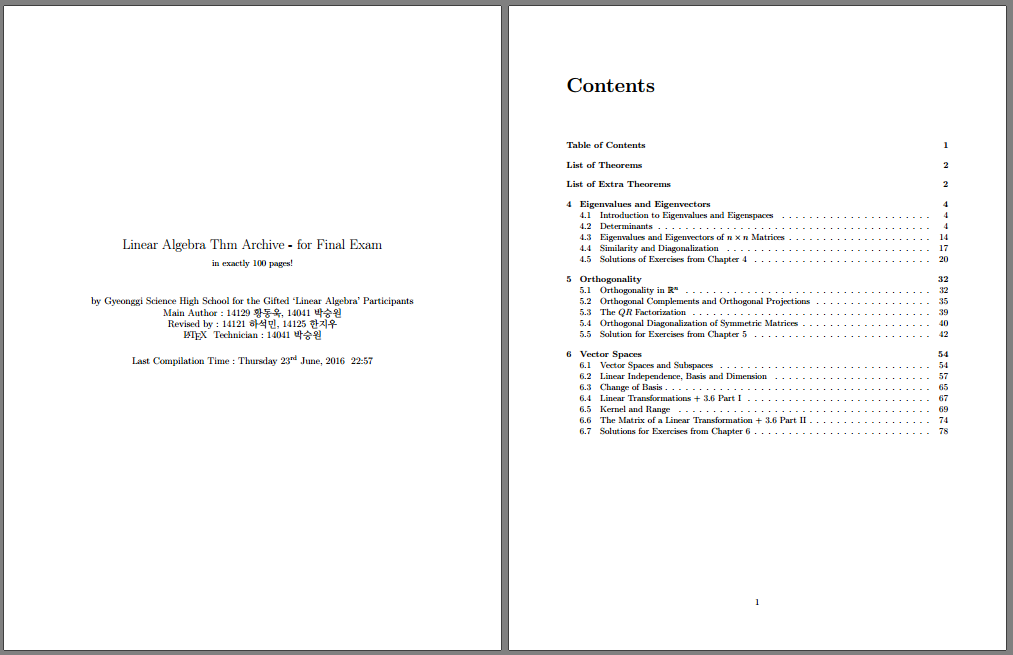
\includegraphics[width=\textwidth]{ex_linearalgebra.png}
	\end{figure}
\end{frame}
\begin{frame}{예시 - 고급물리학 답지}
	\framesubtitle{깔끔한 수식, 그림. By 14041 박승원 + 32기}
	\begin{figure}[h]
		\centering
		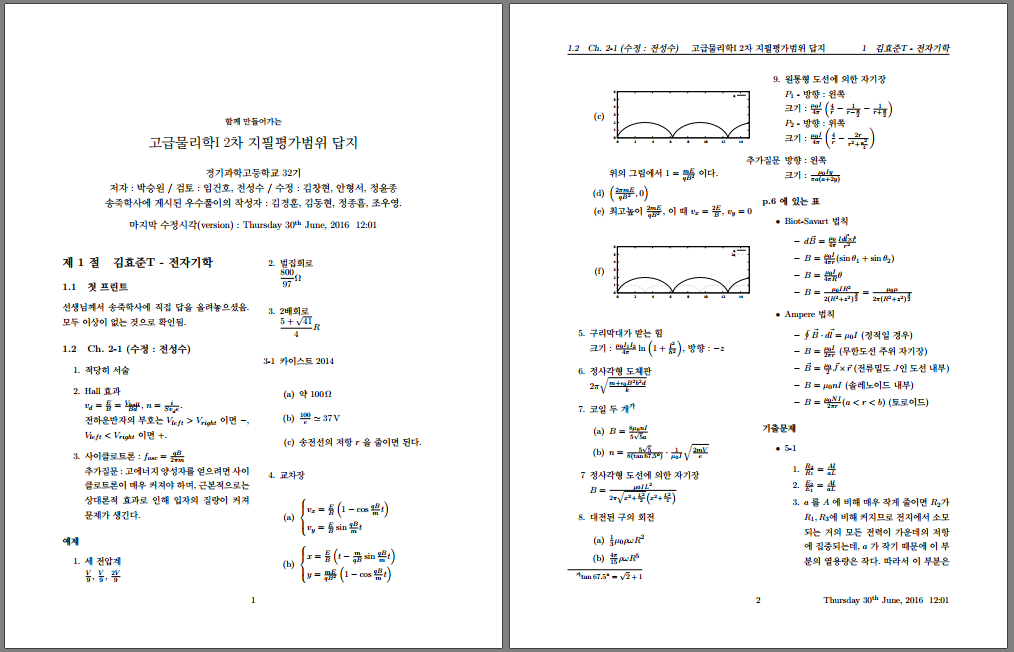
\includegraphics[width=\textwidth]{ex_advphysics.png}
	\end{figure}
\end{frame}
\begin{frame}{예시 - beamer presentation!}
	\framesubtitle{강의자료. By 목진욱 박사님}
	\begin{figure}[h]
		\centering
		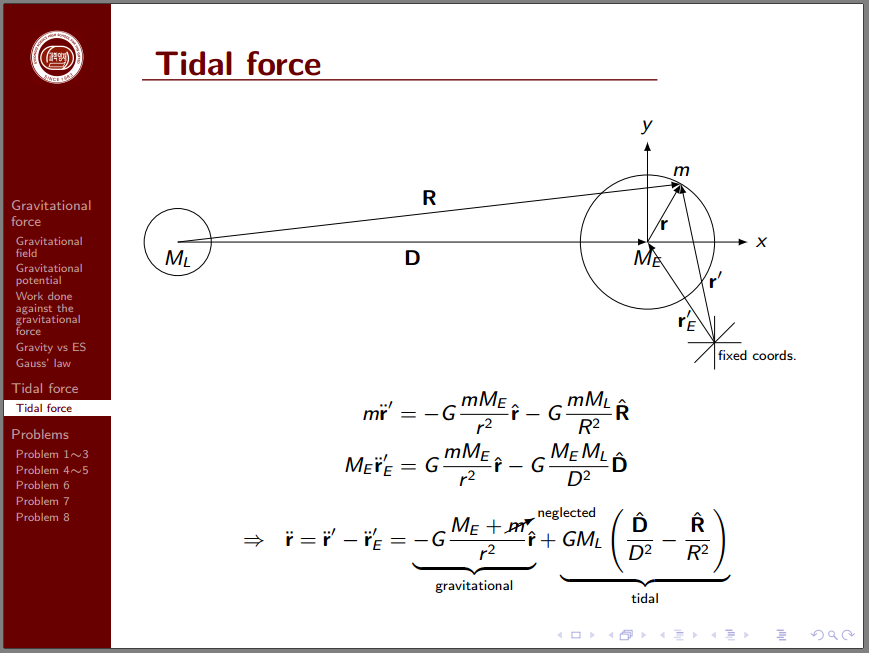
\includegraphics[width=0.9\textwidth]{ex_physicsseminar.png}
	\end{figure}
\end{frame}
\subsection{단점}
\begin{frame}{\LaTeX 의 단점?}
	\begin{itemize}
		\item 非사용자가 읽거나 편집하지 못함
		\begin{itemize}
			\item 가르쳐주면 된다. 
			\item 초반에만 조금 고생하면 된다...
		\end{itemize}
		\item 양식에 맞게 하는 초기 설정이 힘들다. 
		\begin{itemize}
			\item 전문가들에게 맡기자.
			\item 경기과학고 \TeX 사용자협회의 설립취지.
		\end{itemize}
		\item 내가 편집하고 있는게 바로 보이지 않는걸?
		\begin{itemize}
			\item 수식의 경우 거의 실시간으로 inline preview 가능
			\item ... 이건 WYSIWYM 의 숙명
		\end{itemize}
	\end{itemize}
\end{frame}
\end{document} 